\section{Paramètres du processus de conception}
\href{https://youtu.be/6p1QOJi00qQ}{visauliser video}
\begin{itemize}
    \item Les paramètres et les facteurs de conception existent à la fois pour le processus d'ingénierie des systèmes et pour le produit de bus spatial.
    \item Très brièvement, le processus d'ingénierie des systèmes est influencé par des paramètres non techniques tels que :
    \begin{itemize}
        \item la faisabilité de la technologie actuelle,  
        \item l'approche besoins/capacités,  
        \item la disponibilité du financement, et  
        \item les caractéristiques du programme.  
    \end{itemize}
\end{itemize}
\subsection{Caractéristiques du programme}
\begin{figure}[H] % H force l'affichage ici
    \centering
    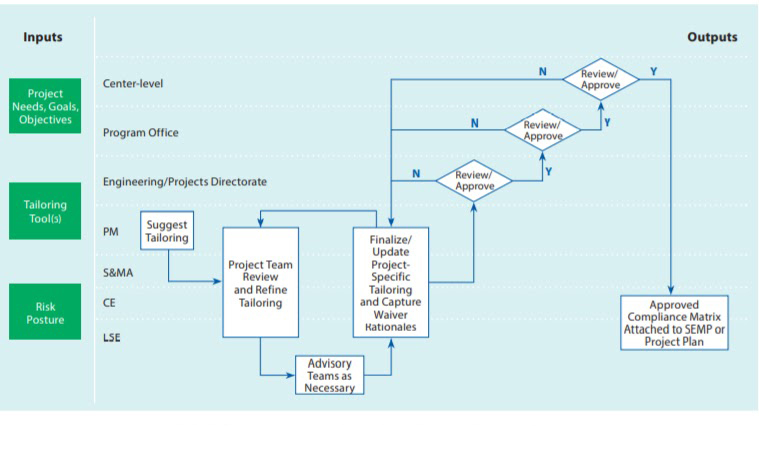
\includegraphics[width=0.8\textwidth]{figures/3.1.jpg}
    \caption{\href{https://www.nasa.gov/wp-content/uploads/2018/09/nasa_systems_engineering_handbook_0.pdf?emrc=4096b9}{Processus de personnalisation des produits de vol spatial national.}}
    \label{fig:communication2}
\end{figure}
Les caractéristiques d’un programme ou d’un projet spatial peuvent être décomposées selon les paramètres suivants :  
\begin{itemize}
    \item \textbf{Type de mission} : Par exemple, les exigences pour une mission habitée sont beaucoup plus strictes que celles d’une petite mission robotique.  
    \item \textbf{Criticité de la mission} dans la réalisation du Plan stratégique de l’Agence : Les missions critiques qui doivent absolument réussir peuvent ne pas être exemptées des exigences NPR (NASA Procedural Requirements).  
    \item \textbf{Niveau de risque acceptable} : Si l’Agence et le client acceptent un risque d’échec plus élevé, certaines exigences NPR peuvent être levées.  
    \item \textbf{Importance nationale} : Un projet ayant une grande importance nationale peut ne pas être exempté des exigences NPR.  
    \item \textbf{Complexité} : Les missions très complexes peuvent nécessiter davantage d’exigences NPR pour assurer la compatibilité des systèmes, tandis que les missions plus simples peuvent être soumises à une rigueur moindre.  
    \item \textbf{Durée de vie de la mission} : Les missions à long terme doivent se conformer plus strictement aux exigences NPR que les programmes/projets de courte durée.  
    \item \textbf{Coût de la mission} : Les missions plus coûteuses peuvent nécessiter une conformité plus stricte aux exigences NPR afin d’assurer un contrôle adéquat du programme/projet.  
    \item \textbf{Contraintes de lancdement} : Si de nombreuses contraintes de lancement existent, un projet peut devoir se conformer davantage aux exigences de l’Agence.  
\end{itemize}
\begin{figure}[H] % H force l'affichage ici
    \centering
    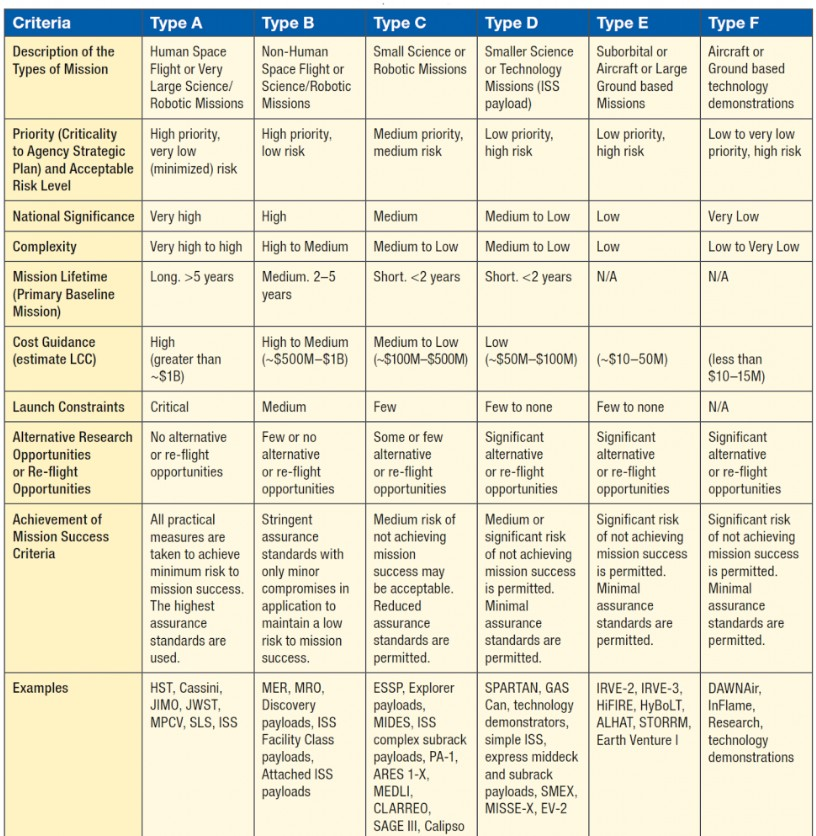
\includegraphics[width=0.8\textwidth]{figures/3.2.jpg}
    \caption{Example of program and project types. Image courtesy of NASA System Engineering Textbook.}
    \label{fig:communication2}
\end{figure}
\begin{itemize}
    \item Pour ce cours, nous nous concentrons sur des programmes similaires au Type D, où les programmes sont :
    \begin{itemize}
        \item de faible priorité,  
        \item à haut risque,  
        \item minimalement complexes,  
        \item de faible importance nationale,  
        \item avec de petits budgets,  
        \item des durées de mission courtes,  
        \item et de nombreuses opportunités alternatives ou de re-lancement.  
    \end{itemize}
    
    \item Les missions CubeSat se situent à l'extrême limite des missions de Type D :
    \begin{itemize}
        \item Les coûts des programmes dirigés par des étudiants dépassent rarement des dizaines de milliers de dollars américains.  
        \item Ces programmes sont principalement éducatifs (faible importance), avec peu ou pas d'exigence de succès.  
        \item Ils se terminent généralement en quelques années.  
    \end{itemize}
    
    \item Les CubeSats sont un excellent moyen de :
    \begin{itemize}
        \item démontrer des \href{https://www.nasa.gov/smallsat-institute/sst-soa}{technologies} de pointe à moindre coût,  
        \item lancer une multitude de satellites pour tester des concepts de détection distribuée,  
        \item offrir des missions innovantes.  
    \end{itemize}
    
    \item Pour les composants du bus spatial qui ne sont pas la charge utile, il existe de nombreuses pièces commerciales disponibles sur le marché (\href{http://www.cubesat.org/}{Commercial Off-The-Shelf, COTS}).  
    
    \item En ce qui concerne le financement :
    \begin{itemize}
        \item Le programme NASA CSLI est probablement la meilleure option pour envoyer votre CubeSat dans l’espace en tant qu’organisation étudiante.  
        \item Le manuel CSLI contient de nombreux conseils pour la rédaction des propositions, comme illustré dans la figure ci-dessus.  
        \item Vous pouvez également obtenir un financement potentiel pour l’achat de matériel ou le financement de la main-d’œuvre via le \href{https://www.nasa.gov/stem/spacegrant/home/Space_Grant_Consortium_Websites.html}{NASA Space Grant Consortium} de votre État.  
    \end{itemize}
\end{itemize}
\begin{itemize}
    \item Le financement participatif est également une option, comme pour les projets \href{https://www.planetary.org/sci-tech/lightsail}{LightSail} ou \href{https://www.kickstarter.com/projects/zacinaction/kicksat-your-personal-spacecraft-in-space}{KickSat}.  
    \item Un financement commercial via le capital-risque est possible si vous avez un modèle économique rentable, comme \href{https://spire.com/}{Spire}.  
\end{itemize}
\begin{figure}[H] % H force l'affichage ici
    \centering
    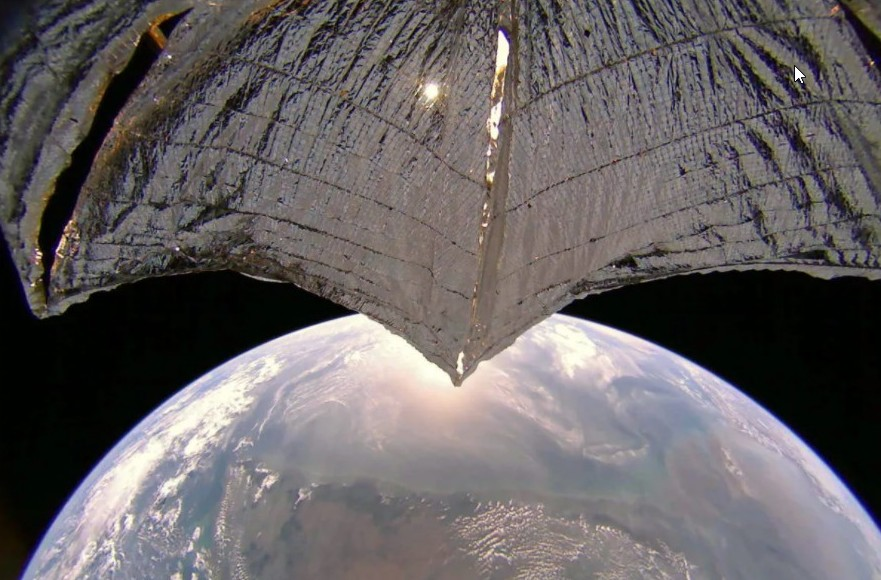
\includegraphics[width=0.8\textwidth]{figures/3.4.jpg}
    \caption{Light Sail 2 over India Light Sail 2 regularly transmits images from its onboard cameras. These images help engineers track the condition of the sail while providing stunning public outreach images. Image courtesy of The Planetary Society}
    \label{fig:communication2}
\end{figure}
\subsection{Processus de révision}
\begin{itemize}
    \item Au cours des différentes revues, trouvez une communauté capable de vous fournir un retour honnête sur votre capacité à respecter la conception de la mission et à gérer le coût et le budget.  
    \item Vous pouvez rejoindre une \href{http://cubesatquestions.slack.com/}{communauté CubeSat sur Slack}, participer aux forums Pressbooks ou solliciter des mentors académiques de votre université.  
    \item Il est essentiel d’avoir des examinateurs qui possèdent des connaissances et une expérience dans votre domaine de spécialisation (science, technologie et/ou éducation), qui peuvent évaluer la nécessité d’une opportunité de vol, qui ont une expertise en vol spatial et en engins spatiaux, mais aussi des compétences générales en développement matériel et en gestion de projet.  
    \item L’un des rôles des examinateurs est d’évaluer la capacité de votre équipe à livrer le satellite à temps et dans le respect du budget.  
    \item Assurez-vous d’inclure votre client dans ce panel d’examen.  
    \item Il est possible d’avoir plusieurs examinateurs afin de couvrir l’ensemble des compétences requises.  
\end{itemize}
\begin{figure}[H] % H force l'affichage ici
    \centering
    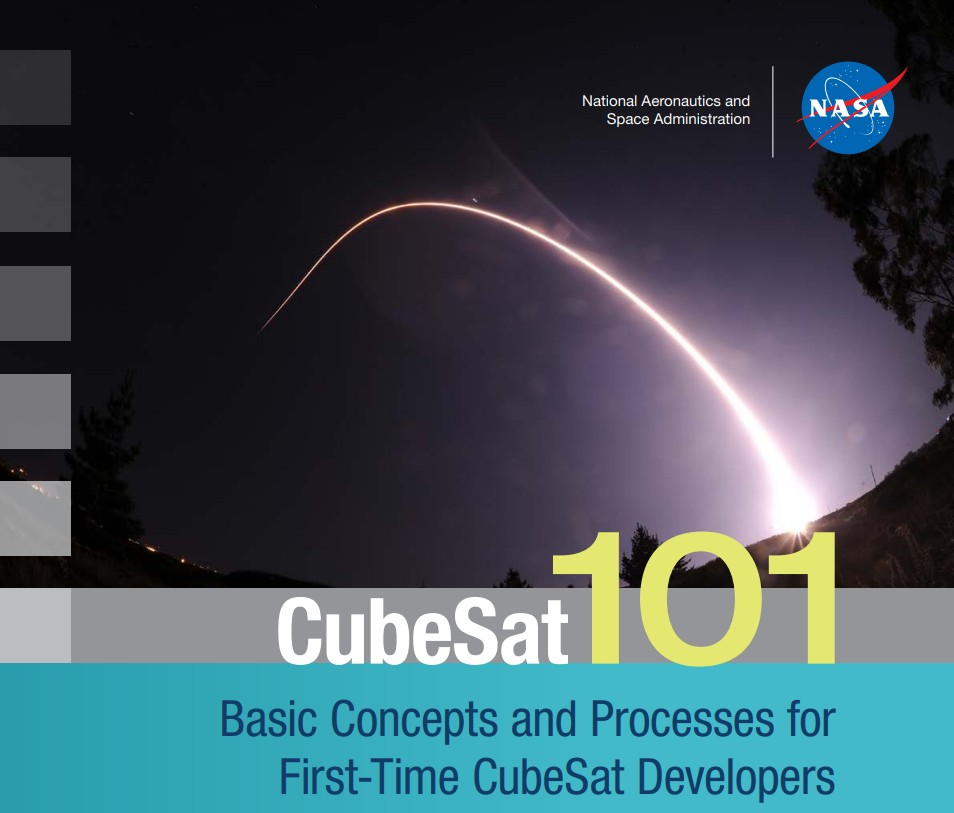
\includegraphics[width=0.8\textwidth]{figures/3.5.jpg}
    \caption{\href{https://www.nasa.gov/wp-content/uploads/2017/03/nasa_csli_cubesat_101_508.pdf}{CubeSat 101. Basic concepts and processes for first-time developers. Image courtesy of NASA.}}
    \label{fig:communication2}
\end{figure}
\subsection{Processus de conception}
\begin{itemize}
    \item Pendant le processus de conception, vous aurez besoin de divers logiciels qui peuvent vous faire gagner du temps et vous permettre d'obtenir de meilleurs résultats plutôt que de réinventer la roue.  
    \item Nous ne mentionnerons que des logiciels gratuits afin de réduire les barrières financières associées à ce projet.  
    \item La conception et l’analyse structurelles mécaniques peuvent être réalisées avec OnShape ou Autodesk Inventor.  
    \item La conception et la simulation des cartes électroniques peuvent être effectuées avec Eagle, KiCAD, \href{http://4pcb.com/}{PCB Artist} et PSpice.  
    \item L'analyse thermique peut être réalisée avec Thermal Desktop.  
    \item La conception et l’analyse d’orbite peuvent être effectuées avec STK.  
    \item Les logiciels de vol peuvent être développés à l’aide de la version open-source du CFS de la NASA, \href{https://github.com/OpenSatKit/OpenSatKit}{OpenSat Kit}.  
\end{itemize}

\textbf{Spécificité du kit Artemis}
\begin{itemize}
    \item Le Hawaii Space Flight Laboratory (HSFL) fournit sa propre suite logicielle appelée COSMOS, incluse avec votre kit.  
    \item Ce logiciel est conçu pour assister la conception de satellites et la planification des missions en intégrant divers outils de simulation, de test et d’opération.  
    \item Tout au long des modules de laboratoire et des tutoriels, COSMOS sera utilisé pour vous guider dans les activités essentielles de conception de satellites.  
    \item Des instructions détaillées étape par étape vous permettront d’apprendre les fonctionnalités et procédures logicielles pertinentes.  
    \item Cette approche structurée garantit une expérience pratique complète en matière de conception, de test et d’exploitation d’un système satellite.  
\end{itemize}
\subsection{Processus de développement}
\begin{itemize}
    \item Pendant le processus d’approvisionnement et de fabrication, vous devrez porter une attention particulière à la façon dont vous vous procurez vos matériaux ainsi qu’à l’équipement nécessaire pour rendre ce matériel apte au vol spatial.  
    \item Le kit Artemis CubeSat devrait être complet et prêt à être lancé tel quel. Si vous souhaitez démontrer une mission entièrement centrée sur le logiciel, vous pouvez ignorer cette section.  
    \item Cependant, si vous souhaitez modifier des composants ou repartir de zéro, sachez que les aspects les plus importants lors du choix du matériel auprès de fournisseurs spécifiques sont :  
    \begin{itemize}
        \item l’aptitude au vol spatial,  
        \item le contrôle des exportations.  
    \end{itemize}
\end{itemize}
\textbf{Composants CubeSat et personnalisation}
\begin{itemize}
    \item Avec la multiplication des \href{http://www.cubesat.org/}{fournisseurs de CubeSat}, la variété des composants commerciaux standard (COTS) permet une plus grande personnalisation et une meilleure adéquation aux exigences techniques.  
    \item En dehors des exigences techniques, les caractéristiques des composants incluent l’héritage spatial, qui est lié au coût, à la main-d'œuvre et aux risques.  
    \item En général, les composants ayant été rigoureusement testés et ayant déjà volé dans l’espace (TRL 9) réduisent le besoin de tests rigoureux et diminuent le risque opérationnel de la mission.  
    \item L’inconvénient des composants qualifiés pour l’espace est leur coût élevé, qui reflète les dépenses liées au développement, aux tests et à la validation en conditions spatiales.  
    \item Plusieurs raisons peuvent justifier l’achat d’un composant COTS auprès d’un fournisseur électronique et la réalisation des tests en interne :  
    \begin{itemize}
        \item Le coût du composant qualifié pour l’espace est trop élevé.  
        \item Le composant non qualifié pour l’espace est mieux adapté aux exigences.  
        \item L’objectif de la mission est de développer un héritage spatial pour ce composant.  
    \end{itemize}
    \item L’inconvénient de faire mûrir la technologie en interne est le coût supplémentaire en main-d'œuvre et en équipement de test, ainsi que le risque accru à gérer.  
    \item Pour les grands projets, la mentalité consiste à minimiser les risques autant que possible, en utilisant souvent des composants qualifiés pour l’espace, ce qui peut conduire à l’utilisation de technologies obsolètes.  
\end{itemize}
\textbf{Spécificités du kit Artemis}
\begin{itemize}
    \item La mentalité des petits projets, comme les CubeSats, est d’accepter et de tolérer un niveau de risque plus élevé, ce qui a guidé l’équipe de conception du kit Artemis CubeSat.  
    \item HSFL dispose de toutes les installations de test nécessaires (table de vibration, chambres à vide thermique, banc de test dynamique et salle blanche) pour réaliser les tests de vérification du kit Artemis CubeSat.  
    \item Aucun des composants n’est qualifié pour l’espace, ce qui nous permet de proposer le kit à un coût très bas. Cependant, tous les composants ont été rigoureusement testés pour garantir leur bon fonctionnement théorique en environnement spatial.  
    \item Si vous ajoutez une charge utile ou modifiez l’un des composants, vous devrez suivre des procédures de test similaires à celles que nous détaillerons dans les chapitres suivants (HSFL est disponible pour fournir un support).  
\end{itemize}

\textbf{Contrôles à l’exportation des États-Unis}

\begin{itemize}
    \item Les réglementations américaines sur l’exportation pour l’industrie spatiale commerciale influencent la composition des équipes en raison de leur impact sur la capacité des membres de différentes nationalités à travailler sur des technologies contrôlées.  
    \item « Le système de contrôle des exportations des États-Unis est conçu pour empêcher la diffusion de technologies sensibles vers des acteurs étrangers pouvant menacer les intérêts américains, tout en permettant aux entreprises américaines de mener des activités commerciales légitimes. Les technologies contrôlées incluent les articles de défense (ex. : missiles), les services de défense (ex. : intégration d’un engin spatial sur un lanceur) et les articles à double usage (ex. : engins spatiaux commerciaux et composants). »  
    \item Il existe deux ensembles de réglementations :  
    \begin{itemize}
        \item \textbf{International Traffic in Arms Regulations (ITAR)} : contrôle les articles, informations ou activités pouvant être utilisés à des fins militaires étrangères, qu’il s’agisse de produits (articles de défense) ou d’assistance (services de défense).  
        \item \textbf{Export Administration Regulations (EAR)} : contrôle les articles et technologies considérés comme à « double usage », c’est-à-dire utilisables à la fois pour des applications commerciales et militaires. La majorité des engins spatiaux commerciaux et de leurs composants relèvent de la juridiction de l’EAR.  
    \end{itemize}
\end{itemize}

\textbf{Spécificités du kit Artemis}

\begin{itemize}
    \item Nous consacrerons une section aux réglementations ITAR et EAR, mais pour le kit Artemis CubeSat, aucun composant n’est soumis à ces réglementations, ce qui signifie que toute personne peut travailler avec les technologies du kit.  
\end{itemize}
